\documentclass[
aps,%
12pt,%
final,%
notitlepage,%
oneside,%
onecolumn,%
nobibnotes,%
nofootinbib,%
superscriptaddress,%
noshowpacs,%
centertags]%
{revtex4}


\usepackage{subfigure}

\usepackage{bm}
\usepackage{amsmath}
\usepackage{amssymb}
\usepackage{array}
\usepackage{graphicx}
\usepackage{caption2}






\begin{document}
\title{Generation of non-maximally entangled states between BECs with quantum optimal control methods}

\author{Ilia D. Lazarev}
\affiliation{Federal Research Center of Problems of Chemical Physics and Medicinal Chemistry RAS, Acad. Semenov av. 1, Chernogolovka, Moscow region, Russia, 142432}

\author{Alexey N. Pyrkov}
\email{pyrkov@icp.ac.ru}
\affiliation{Federal Research Center of Problems of Chemical Physics and Medicinal Chemistry RAS, Acad. Semenov av. 1, Chernogolovka, Moscow region, Russia, 142432}

%\date{today}


\begin{abstract}

In the last decade, different theoretical methods for entanglement generation between distant BEC qubits (macroscopic cold atomic ensembles) were proposed. However, experimental realization of such states is still challenging beside some special cases. The most theoretically investigated entangled states between macroscopic BECs are non-maximally entangled states obtained with $SzSz$ entangling Hamiltonian. With the use of such states, the protocols for quantum teleportation, remote state preporation and many others were developed for macroscopic qubits on the basis of BECs. Here we show that it is possible to obtain such states with the use of the bosonic analog of $XY$ Hamiltonian and the methods of quantum optimal control. We compare performance of this scheme in the meaning of fidelity and entanglement for different drift and control Hamiltonians. We use the well-established QuTip open python library for all calculations.

\end{abstract}

\maketitle

\section{Introduction}

Entanglement serves as a crucial asset for various quantum technologies, including quantum computing, quantum communication, and quantum metrology. The observation of entangled states, indicative of nonlocality and a fundamental distinction between quantum and classical physics, becomes particularly intriguing when witnessed in macroscopic objects that conventionally exhibit classical behavior. Consequently, significant endeavors have been directed towards detecting such states in multipartite and massive systems, such as optomechanical devices \cite{Galland2014,SafaviNaeini2014} or Bose-Einstein condensates (BECs) \cite{Duan2000,Pu2000,pyrkov2013}. BECs stand out as excellent candidates for studying entanglement in quantum macroscopic systems. In these ensembles, the internal states of the atoms collectively form a spin. While extensive theoretical and experimental investigations have focused on the generation of entangled states with squeezing in single-spin systems, the corresponding idea of two-mode squeezing in the context of spins has received comparatively less attention. However, diverse nonclassical collective spin states can be engineered, including different spin-squeezed states \cite{kitagawa1993squeezed}, twin-Fock states \cite{Luecke2011}, and two-mode squeezed (TMS) states \cite{Baumgarten2008}. Investigating the two-spin version of one-axis squeezing, researchers in Refs. \cite{pyrkov2013,byrnes2013fractality} unveiled a complex entanglement structure with time-dependent fractal characteristics. Numerous studies have explored methods to generate this specific state \cite{pyrkov2013,2014Entanglement,kurkjian2013spin}, while other investigations have delved into the creation of various types of entangled states \cite{pettersson2017light,bec7}. Notably, significant research on the two-spin scenario has been conducted in the realm of atomic ensembles, particularly led by the Polzik research group \cite{julsgaard2001experimental,Krauter_2013}. In these studies, although the physical system comprises an atomic ensemble, the analysis primarily revolves around a regime where the behavior of spin variables can be approximated using bosonic modes, employing the Holstein-Primakoff transformation. Within this approximation, the resultant entangled state can be characterized as a two-mode squeezed state.  For Bose-Einstein condensates (BECs), the creation of many-particle entanglement localized in a single spatial location \cite{sorensen2001many,Augusto2014Fisher} and spatially separate regions \cite{kunkel2018spatially,lange2018entanglement,fadel2018spatial} within one BEC condensate has
been observed. Furthermore, following the identification of a multipartite Bell inequality involving low-order correlators \cite{Tura2014}, instances of Bell correlations have been experimentally confirmed in a BEC \cite{schmied2016bell} and a thermal atomic ensemble \cite{engelsen2017}. Notably, these validations stem from the violation of a practically applicable witness that exclusively involves collective spin measurements. Recently, an experiment successfully demonstrated the achievement of entanglement between two spatially separated BECs \cite{Colciaghi2023}. However, in many protocols of quantum information processing on the basis of macroscopic BEC qubits (such as quantum teleportation, remote state preparation and so on) some special class of non-maximally entangled states generated with $SzSz$-Hamiltonian is used \cite{BYRNES2015102,pyrkov2014quantum,pyrkov2014full,manish2021} and it is worth to understand how to produce such states in other settings.

In a recent demonstration, quantum optimal control methods were employed to prepare states of atomic ensembles and Bose-Einstein condensates (BECs) in optical lattices \cite{Dupont2021}. Specifically, a one-dimensional optical lattice was created using two counter-propagating laser beams with identical wavelengths but differing phases. The experiment involved loading a BEC of ultra-cold 87Rb atoms into this lattice. To dynamically manipulate the optical lattice and guide the quantum system to a desired target state, a gradient-based optimal control algorithm was utilized. This algorithm calculated the optimal phase adjustment that effectively "shook" the optical lattice back and forth. As a result, at the conclusion of the control process, the atoms existed in a well-defined superposition of speeds, each being a multiple of an elementary speed. Notably, this process allowed for the creation of specific patterns.

In this study, we examine the bosonic counterpart of the $XY$-Hamiltonian, giving rise to the two-axis two-spin squeezed (2A2S) state \cite{bec4}. Our investigation reveals the potential to generate the non-maximally entangled states in Bose-Einstein Condensates (BECs) by leveraging this Hamiltonian and employing quantum optimal control techniques. Through a comparative analysis, we demonstrate that optimal control enables precise parameter tuning to achieve these non-maximally entangled states, as opposed to relying solely on the drift Hamiltonian. All calculations are performed using the established QuTip open-source Python library. The paper is structured as follows: Section 2 provides an overview of qubit encoding to BECs and the generation of non-maximally entangled states between BECs, essential for the generalization of quantum information protocols with BECs; Section 3 delves into the core concept of the quantum optimal control approach, specifically focusing on the GRAPE algorithm and also entails a comparative analysis of different schemes for attaining non-maximally entangled states using the bosonic analog of the $XY$-Hamiltonian and quantum optimal control methods. Finally, our results are summarized in Section 4.


\section{Encoding qubit into a macroscopic BEC and non-maximally entangled states}

The system under consideration comprises two neutral atomic ensembles or Bose-Einstein Condensates (BECs). Each atom within these ensembles possesses two pertinent internal states. A typical selection for these internal states involves hyperfine ground states, exemplified by the $ F= 1, m_F = - 1 $ and $ F = 2, m_F = 1 $ states, as observed in the case of of $^{87}$Rb (Pezzè et al., 2018). Denote the bosonic annihilation operators of the two states as $ a $ and $ b $, obeying commutation relations $ [a,a^\dagger]= [b,b^\dagger]= 1 $ \cite{li2009spin}. We encode a standard qubit state $ \alpha | 0 \rangle + \beta |1 \rangle $ in the BEC in the state
%
\begin{equation}
\label{singlequbitstate}
|\alpha, \beta \rangle \rangle \equiv \frac{1}{\sqrt{N!}} \left( \alpha a^\dagger + \beta b^\dagger \right)^N |0 \rangle ,
\end{equation}
%
where $ \alpha $ and $ \beta $ are arbitrary complex numbers satisfying $ |\alpha |^2 + | \beta |^2 = 1 $
(double brackets are used to denote the bosonic qubit states).  For simplicity let us first consider the boson number $ N = a^\dagger a + b^\dagger b $ to be a conserved number. Each qubit state is therefore encoded by $ N $ bosonic particles with a collective Hilbert space dimension of $ N+1 $.

The state (\ref{singlequbitstate}) can be visualized by a vector on the Bloch sphere with an angular representation
$ \alpha = \cos(\theta/2) , \beta=\sin(\theta/2) e^{i\phi} $.  The state $ |\alpha, \beta \rangle \rangle $ can be manipulated using Schwinger boson (Stokes operators) operators
\begin{align}
 S^x = a^\dagger b + b^\dagger a ,\nonumber \\
 S^y = -i a^\dagger b + i b^\dagger a, \nonumber \\
 S^z = a^\dagger a - b^\dagger b ,
\end{align}
%
which satisfy the usual spin commutation relations $ [S^i,S^j] = 2i \epsilon_{ijk} S^k $, where
$ \epsilon_{ijk} $ is the Levi-Civita antisymmetric tensor.  In the spin language, (\ref{singlequbitstate}) forms a spin-$ N/2 $ representation of the SU(2) group (we omit the factor of 2 in our spin definition for convenience).  Single qubit rotations can be executed in a manner entirely analogous to conventional qubits. To illustrate, rotations along the $z$-axis of the Bloch sphere can be achieved through a process of evolution
%
\begin{align}
e^{-i \Omega S^z t} |\alpha, \beta \rangle \rangle & =
\frac{1}{\sqrt{N!}} \sum_{k=0}^N \binom{N}{k} ( \alpha a^\dagger e^{-i\Omega t})^k ( \beta b^\dagger e^{i \Omega t})^{N-k} |0 \rangle \nonumber \\
& = |\alpha e^{-i \Omega t}, \beta e^{i \Omega t}\rangle \rangle .
\end{align}
%
Similar rotations may be performed around any axis by an application of
%
\begin{align}
H_{1} = \hbar \Omega \bm{n} \cdot \bm{S} =  \hbar \Omega ( n_x S^x + n_y S^y +n_z S^z )
\end{align}
%
where $ \bm{n} = (n_x,n_y,n_z) $ is a unit vector. Experimental result from work of Ref.\cite{treutlein2006quantum} on single qubit rotations are presented in Fig.\ref{fig1:entanglement}. The transition $|0,1\rangle\rangle \leftrightarrow |1,0\rangle\rangle$ is driven by a microwave $\nu_\mathrm{mw}$ and a radio-frequency $\nu_\mathrm{rf}$. Expectation values of the spin are similar to that of a single spin (up to a factor of $ N $), exhibiting values
%
\begin{align}
\langle S^x \rangle & = N(\alpha^* \beta + \alpha \beta^*) \nonumber \\
\langle S^y \rangle & = N(-i \alpha^* \beta + i \alpha \beta^*) \nonumber \\
\langle S^z \rangle & = N( | \alpha |^2 - | \beta |^2 ) .
\end{align}
%
The variance of the spins, however, decreases in comparison to the maximum amplitudes
%
\begin{align}
\label{variance}
\frac{\langle (S^z)^2 \rangle - \langle S^z \rangle^2}{N^2} = \frac{4 |\alpha \beta |^2}{N}
\end{align}
%
in accordance to widespread notion that for $ N \rightarrow \infty $ the spins approach classical variables. We shall however see in the following section that despite the classical appearance of such a state, such a many boson state can exhibit quantum properties such as entanglement.

The quantum state of a single qubit in (\ref{singlequbitstate}) can be considered to be ``duplicated'' over $ N $ bosons, which are all in the same state.  Thus although many physical particles encode the quantum state, the Hilbert space mapping is one-to-one.  In this sense, the encoding presented here has similarities with quantum error correcting codes where an expanded Hilbert space is used to encode quantum states.

\subsection{Two qubit BEC entanglement}

Two qubit gates can be formed by any product of the Schwinger boson operators of the form
%
\begin{align}
H_2 = \sum_{i,j = x,y,z} \hbar \Omega_{i j} S^{i}_1 S^{j}_2
\end{align}
%
where $ \Omega_{i j} $ are real symmetric parameters. The combination of $ H_1 $ and $ H_2$ may be combined to form an arbitrary Hamiltonian involving spin operators according to universality arguments \cite{lloyd95}. By successive commutations an arbitrary product of spin Hamiltonians
%
\begin{align}
\label{generaltwoqubit}
H \propto \prod_{n=1}^M (S^j_n)^{m(n)}
\end{align}
%
may be produced, where $ M $ is the total number of qubits, $ j = x,y,z $, and $ m(n) = 0,1 $. Although in general
higher order operators may be constructed (e.g. $ m(n) \ge 2$), our aim here is to simulate the standard qubit system using the BEC qubits. Since for Pauli operators $ (\sigma^j)^2 = 1 $, such higher order operators are unnecessary for our purposes.

A key difference between Pauli operators and the Schwinger boson operators are that $ \sigma^j \sim O(1) $, whereas $ S^j \sim O(N) $.  This makes the two qubit interaction $ H_2 \sim O(N^2) $.  The consequence of the boosted energy scale of the interaction can be observed by examining explicitly the state evolution of two qubits. For simplicity, let us consider henceforth consider the interaction Hamiltonian
%
\begin{align}
\label{zzham}
H_2 = \hbar \Omega S^z_1 S^z_2 .
\end{align}
%
This may be done without any loss of generality since (\ref{generaltwoqubit}) can be converted to (\ref{zzham}) by universality arguments.
As a simple illustration, let us perform the analogue of the maximally entangling operation
%
\begin{align}
& e^{-i  \sigma^z_1 \sigma^z_2 \frac{\pi}{4} } ( | \uparrow \rangle + | \downarrow \rangle ) ( | \uparrow \rangle + | \downarrow \rangle ) =  | + y \rangle | \uparrow \rangle  + | - y \rangle | \downarrow \rangle, \label{qubitentangler}
\end{align}
%
where $ | \pm y \rangle = e^{\mp i\frac{\pi}{4}} | \uparrow \rangle + e^{\pm i\frac{\pi}{4}} | \downarrow \rangle $. Starting from two unentangled qubits, we may apply $ H_2 $ to obtain
%
\begin{align}
& e^{-i \Omega S^z_1 S^z_2 t} | \frac{1}{\sqrt{2}}, \frac{1}{\sqrt{2}} \rangle \rangle | \frac{1}{\sqrt{2}}, \frac{1}{\sqrt{2}} \rangle \rangle \nonumber \\
& = \frac{1}{\sqrt{2^N}} \sum_{k_2} \sqrt{\binom{N}{k_2}}  | \frac{e^{i(N-2 k_2)\Omega t}}{\sqrt{2}}  , \frac{e^{-i(N-2 k_2) \Omega t}}{\sqrt{2}}  \rangle \rangle |k_2 \rangle ,
\label{bosonqubitentanglement}
\end{align}
%
where we have introduced normalized eigenstates of the $ S^z $ operator $ |k \rangle \equiv \frac{(a^\dagger)^k (b^\dagger)^{N-k}}{\sqrt{k!(N-k)!}} |0 \rangle $.  For gate times equal to $ \Omega t = \pi/4N   $ we obtain the analogous state to (\ref{qubitentangler}). For example, the maximum $z$ eigenstates $ |k_2=0,N \rangle $ on qubit 2 are entangled with the states

\begin{equation}
| \pm y \rangle \rangle \equiv | \frac{e^{\pm i\pi/4}}{\sqrt{2}}  , \frac{e^{\mp i \pi/4}}{\sqrt{2}} \rangle \rangle  ,
\end{equation}
which is the analogue of a Bell state for the bosonic qubits. A visualization of the state (\ref{bosonqubitentanglement}) is shown in Figure \ref{fig1:entanglement}c. For each $z$-eigenstate on qubit 2, there is a state


\begin{equation}
    | \frac{e^{i(N-2 k_2) \pi/4N}}{\sqrt{2}}  , \frac{e^{-i(N-2 k_2) \pi/4N}}{\sqrt{2}} \rangle \rangle
\end{equation}
%
on qubit 1 represented on the Bloch sphere entangled with it. The type of entangled state is a continuous version of the original qubit sequence (\ref{qubitentangler}), and has similarities to continuous variable formulations of quantum computing \cite{braunstein2005quantum}, although the class of states that are used here are quite different.

The two-axis two-spin (2A2S) Hamiltonian is then defined as
%
\begin{align}
H = H_{2A2S} = \frac{J}{2} (S_1^x S_2^x - S_1^y S_2^y) = J(S_1^+ S_2^+ + S_1^-S_2^-) ,
\label{eq:Hamiltonian}
\end{align}
%
where
%
\begin{align}
S_j^{+} & = \frac{1}{2} (S_j^x + i S_j^y) = b_j^\dagger a_j \nonumber \\
S_j^{-} & =  \frac{1}{2}  (S_j^x - i S_j^y)= a_j^\dagger b_j ,
\end{align}
%
and $ J $ is an energy constant. This is a straightforward generalization of the two-axis one-spin (2A1S) countertwisting Hamiltonian studied by Kitagawa and Ueda \cite{kitagawa1993squeezed}
%
\begin{align}
H_{2A1S} = \frac{J}{2} [ (S^x)^2  - (S^y)^2 ] = J[ (S^+)^2 + (S^-)^2 ] .
\end{align}
%

\section{Quantum optimal control of entangled states between BECs}

Fundamental inquiries in the realm of engineering quantum technological devices include "which states are attainable?" or "what quantum gates can be executed?". Quantum optimal control address these questions establishing a crucial link between engineering considerations and the foundational principles of mathematical control theory.

\subsection{State-to-state control}

Suppose that our system is described by a Hamiltonian

\begin{align}
\hat{H}(t) = \hat{H}_0 + \sum_{i=1}^{n} u_i(t) \hat{H}_i
\end{align}

We define the time-independent component of the Hamiltonian as $\hat{H}_0$, referred to as the drift. The fields $u_i(t)$ represent the controls, and $\hat{H}_i$ denotes the control Hamiltonians. In contexts such as atomic physics, $\hat{H}_0$ characterizes the energy level structure of the system, while $u_i(t)$ corresponds to laser or microwave fields, and $\hat{H}_i$ represents dipole operators describing various field modes.



Our objective is to initiate from an initial state $|\psi_0\rangle$ at time $t = 0$ and determine controls such that we attain the state $|\psi_1\rangle$ at $t = T$. In quantum physics, the global phase is inconsequential, aligning with the goal of maximizing the overlap $J = |\langle \psi_1 | \psi(T)\rangle|^2$.

The dynamics of our system is described with the Schrödinger equation:

$$i \frac{\partial}{\partial t} |\psi(t)\rangle = \hat{H}(t) |\psi(t)\rangle$$.

In order to find the optimal $u_i(t)$ the GRadient Ascent Pulse Engineering (GRAPE) algorithm \cite{Khaneja2005} can be used. The GRAPE can be described as following: 1) Many practical generators for control pulses often represent pulses in a piecewise constant fashion. Thus it is possible to chop the total time into intervals of length $\delta t = T/N$. 2) The formal solution of the Schrödinger equation is then expressed in terms of a product of unitary operators, each associated with a specific time interval and controlled by the corresponding pulse parameters. 3) The performance index is introduced and expressed in terms of the overlap of propagated and back-propagated quantum states. The objective is to maximize this performance index. 4) The optimization involves the calculation of gradients at each time step. The analytical derivation of these gradients is facilitated by the use of the derivative of an exponential, allowing for efficient updates of the control parameters. 5) The controls are updated iteratively based on the gradient, aiming to extremalize the performance index. We used this algorithm for generation and optimizing special type of entangled states between macroscopic BEC qubits.

\subsection{Entanglement generation between BECs with quantum optimal control}

Here we model and analyze the methods of quantum optimal control for preparation of special set of entangled states between BECs. This set of entangled states consist of non-maximally entangled states that have the characteristic ‘devil’s crevasse’ form which arises from a $SzSz$ interaction, giving a non-zero entanglement for all time except the states equivalent to the initial product state. This specialized set of entangled states proves highly practical in various quantum information processing applications, including but not limited to quantum teleportation, remote state preparation, and the establishment of quantum networks. In this study, we design such states from bosonic analog of $XY$-Hamiltonian with methods of quantum optimal control. We consider the two-axis two-spin (2A2S) Hamiltonian $$H = H_{2A2S} = \frac{J}{2} (S_1^x S_2^x - S_1^y S_2^y)$$ as a drift Hamiltonian  starting from the initial state $$| \frac{1}{\sqrt{2}}, \frac{1}{\sqrt{2}} \rangle \rangle | \frac{1}{\sqrt{2}}, \frac{1}{\sqrt{2}} \rangle \rangle$$ convert it to the following non-maximally entangled state from (\ref{bosonqubitentanglement}) which is shown in Figure~\ref{fig1:entanglement}c with the use of different control Hamiltonians $S_1^{x,y}$,$S_2^{x,y}$,$(S_1^x S_2^x - S_1^y S_2^y)$, $S_1^x S_2^x$, $S_1^y S_2^y$, $(S^z)^2$ and their combinations.
In order to realize that we use the well-established QuTIP library \cite{qutip}. All calculations are implemented on Intel(R) Core(TM) i9-9900 CPU @ 3.10GHz (8 cores / 16 threads) with 64GiB RAM. The results are presented on the Figures~\ref{fig2:rotation}, \ref{fig3:time-depended} and \ref{fig4:squeezing}.

From Figure~\ref{fig2:rotation}, it is evident that the controls associated with $S_1^y$ and $S_2^y$ exhibit negligible influence on the initial state dynamics when compared to the impact of the drift Hamiltonian itself. This observation holds true for both fidelity and entanglement metrics. Conversely, controls corresponding to $S_1^x$ and $S_2^x$ contribute to an enhancement in fidelity, albeit at the expense of entanglement. This phenomenon may be attributed to the nonlinear behavior of entanglement characterized by the 'devil’s crevasse' pattern during evolution.


The control over the interaction term, specifically $(S_1^x S_2^x - S_1^y S_2^y)$, proves to be beneficial, leading to improvements in both fidelity and entanglement generation between Bose-Einstein Condensates (BECs) in comparison to relying solely on the pure drift Hamiltonian (see Figure~\ref{fig3:time-depended}a). Further enhancements can be achieved by introducing rotations of both BECs around the $x$-axis (see Figures~\ref{fig3:time-depended}b and Figures~\ref{fig3:time-depended}c). As an illustrative example, artificial controls involving two-spin one-axis squeezings, such as $S_1^x S_2^x$ and $S_1^y S_2^y$, exhibit smooth and nearly ideal dynamics toward the target state, although their practical implementation may pose challenges in experimental settings (see Figure~\ref{fig3:time-depended}d).

The Figure \ref{fig4:squeezing} depicts cases where quantum optimal control results in almost perfect generation of 'devil’s crevasse' entangled states. Notably, one-axis one-qubit squeezings $(S_{1,2}^z)^2$ serve as effective controls in this context. The the interaction drift Hamiltonian and squeezing controls complement each other, proving feasible for potential experimental realization and achieving nearly perfect convergence.

%%

\section{Conclusion}

In this study we investigated quantum optimal control methods for generating a specific set of entangled states between Bose-Einstein Condensates (BECs). These states, characterized by a distinctive 'devil’s crevasse' pattern produced from $SzSz$ interaction. The design of quantum optimal control experiments involves utilizing the bosonic analog of the $XY$-Hamiltonian, the two-axis two-spin (2A2S) Hamiltonian, for obtaining such states.

The study emphasizes the beneficial impact of quantum optimal control methods which enhances both fidelity and entanglement generation compared to relying solely on the drift Hamiltonian. Controls associated with the rotations  contribute to fidelity improvement but at the expense of entanglement, reflecting nonlinear entanglement behavior during evolution. Controls with interaction terms and two-spin one-axis squeezing show very good convergence toward the target state, although practical implementation challenges may arise. The one-axis one-qubit squeezings are effective controls for achieving almost perfect generation of 'devil’s crevasse' entangled states, showcasing potential for experimental realization and nearly perfect convergence. Thus this investigation pave a way for more presice generation and design of entangled states between BECs.

\section{ACKNOWLEDGMENTS}
This work is supported by Russian Science Foundation (grant no 23-21-00507).

\bibliographystyle{apsrev}
\bibliography{biblio}

\newpage

\begin{figure*}[t!]
\setcaptionmargin{5mm}
\onelinecaptionsfalse
\begin{center}
    \includegraphics[width=13cm]{fig1.eps}
\end{center}
\captionstyle{normal}
\caption{
    {\bf a} The entanglement normalized to the maximum entanglement ($E_{\mbox{\tiny max}} = \log_2 (N+1) $) between two bosonic qubits for the particle numbers as shown.
    {\bf b} Entanglement at a time $ \Omega t= \pi/4N $ for various boson numbers $ N $.
    {\bf c} A schematic representation of the entangled state (\ref{bosonqubitentanglement}).
}
\label{fig1:entanglement}
\end{figure*}

\newpage

\begin{figure*}[t!]
\setcaptionmargin{5mm}
\onelinecaptionsfalse
\subfigure{%
   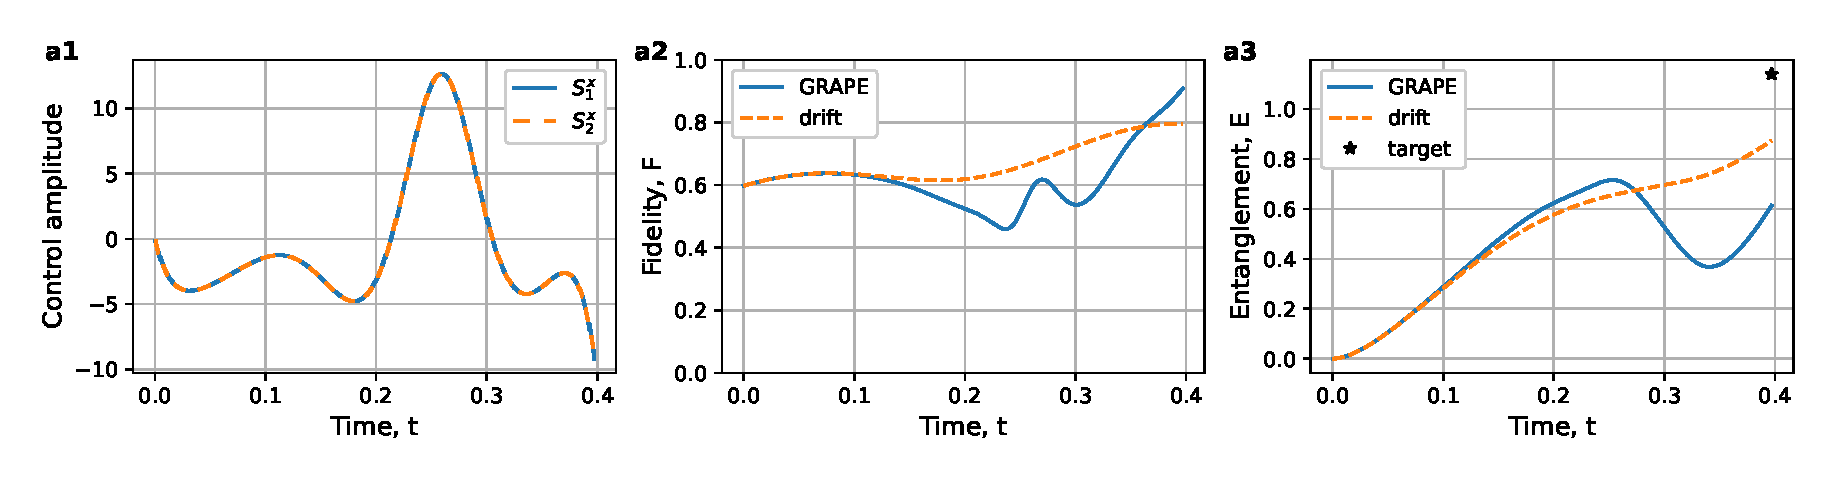
\includegraphics[width=0.92\textwidth]{fig2a.eps}
}
\subfigure{%
   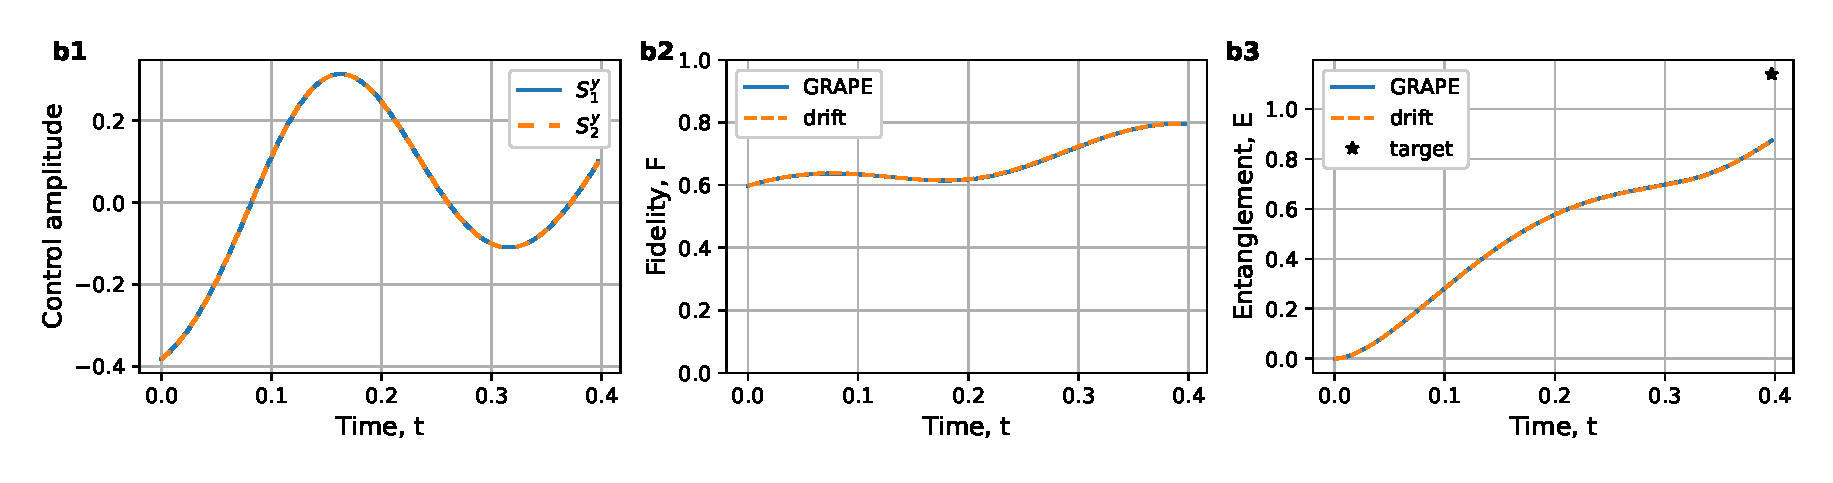
\includegraphics[width=0.92\textwidth]{fig2b.eps}
}
\captionstyle{normal}
\caption{
    Optimal control with local rotation {\bf a} around $X$~-~axis and {\bf b} around $Y$~-~axis as controls. Amplitudes of the controls in controlled Hamiltonian are depicted in the left column {\bf a1} and {\bf b1}. Same qubit controls have similar amplitudes. A fidelity between the target state~(\ref{bosonqubitentanglement}) for $t=\frac{2}{5\Omega}$ and final state under the drift Hamiltonian itself and the full Hamiltonian obtained with GRAPE are depicted in the middle column {\bf a2} and {\bf b2}. Corresponded entanglement evolutions are depicted in the right column {\bf a3} and {\bf b3}.
}
\label{fig2:rotation}
\end{figure*}

\newpage

\begin{figure*}[t!]
\setcaptionmargin{5mm}
\onelinecaptionsfalse
\subfigure{%
   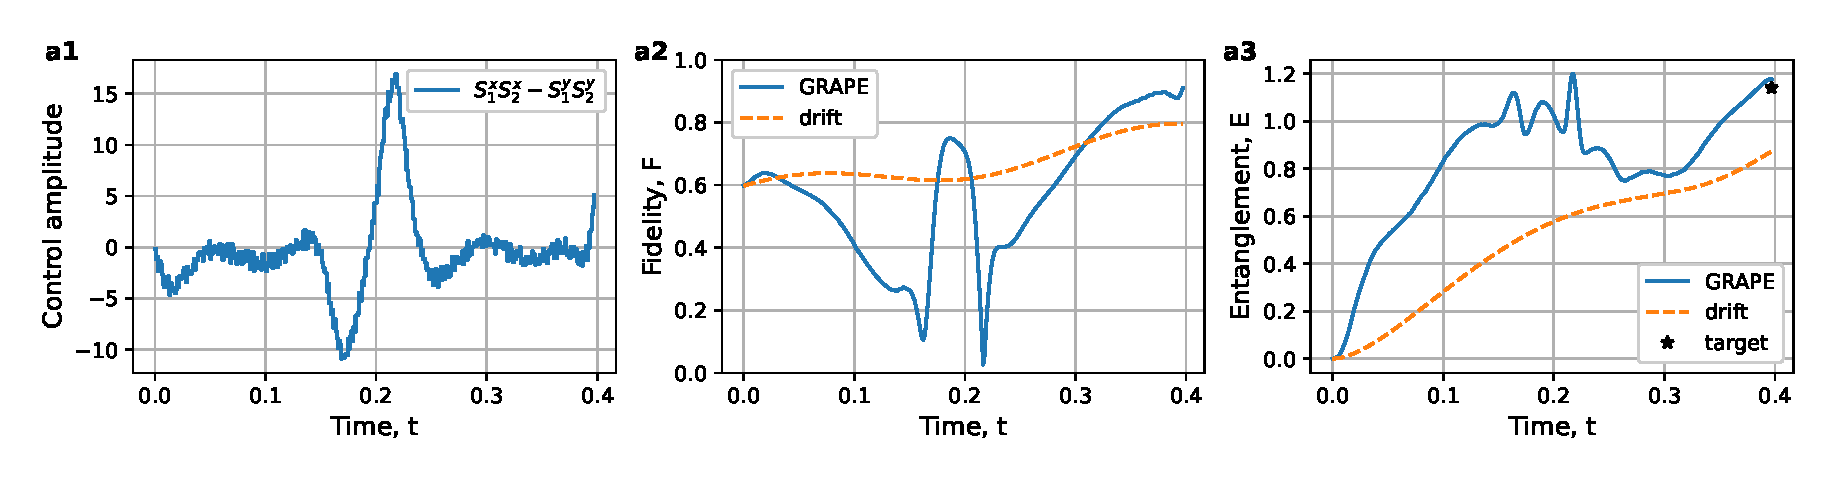
\includegraphics[width=0.92\textwidth]{fig3a.eps}
}
\subfigure{%
   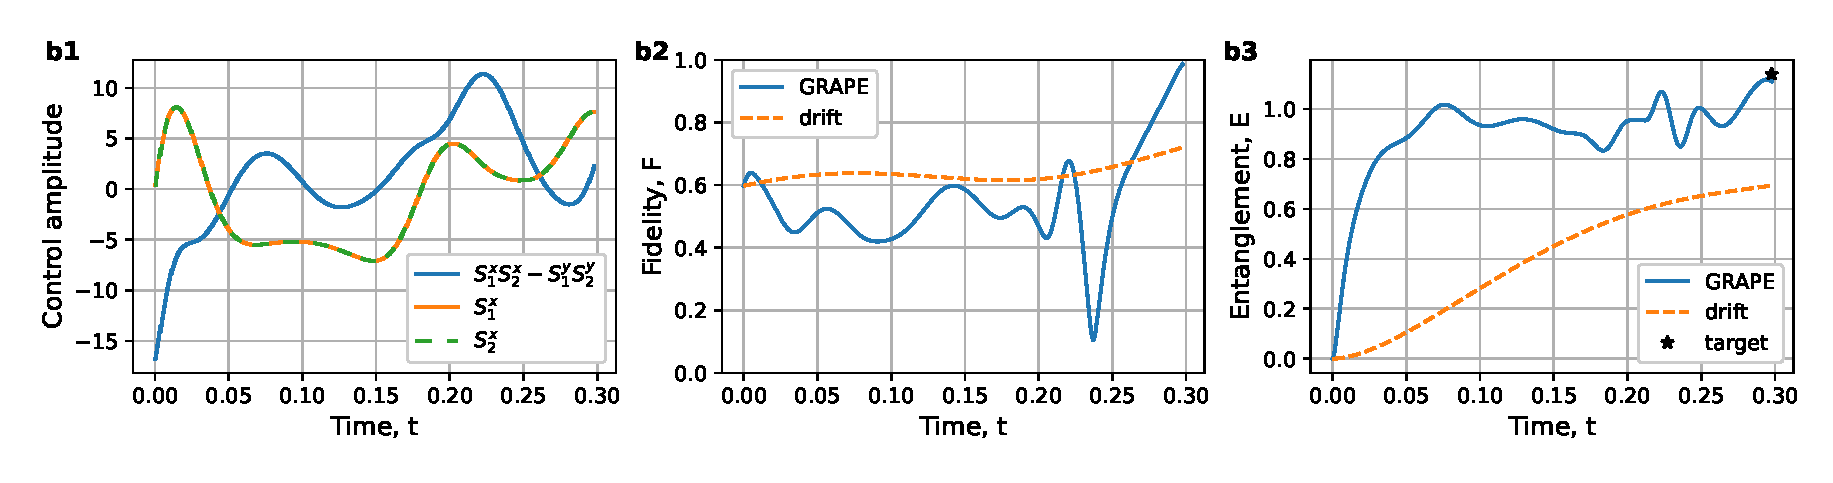
\includegraphics[width=0.92\textwidth]{fig3b.eps}
}
\subfigure{%
   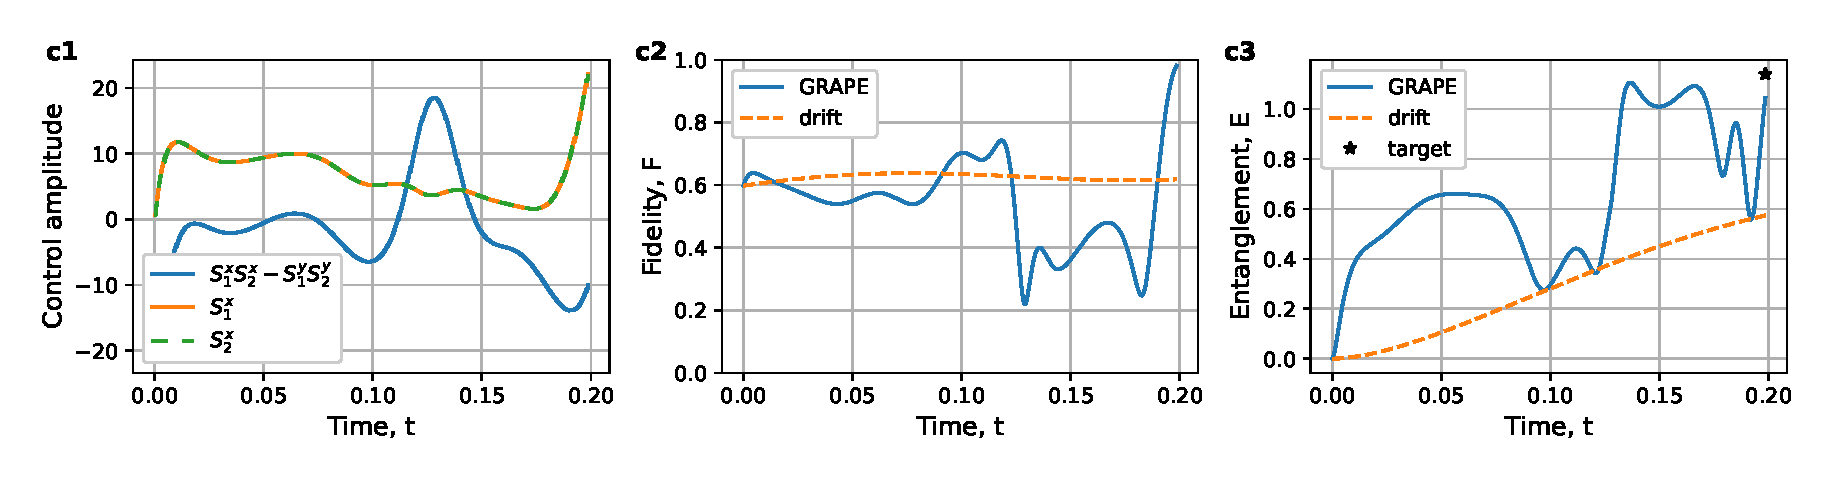
\includegraphics[width=0.92\textwidth]{fig3c.eps}
}
\subfigure{%
   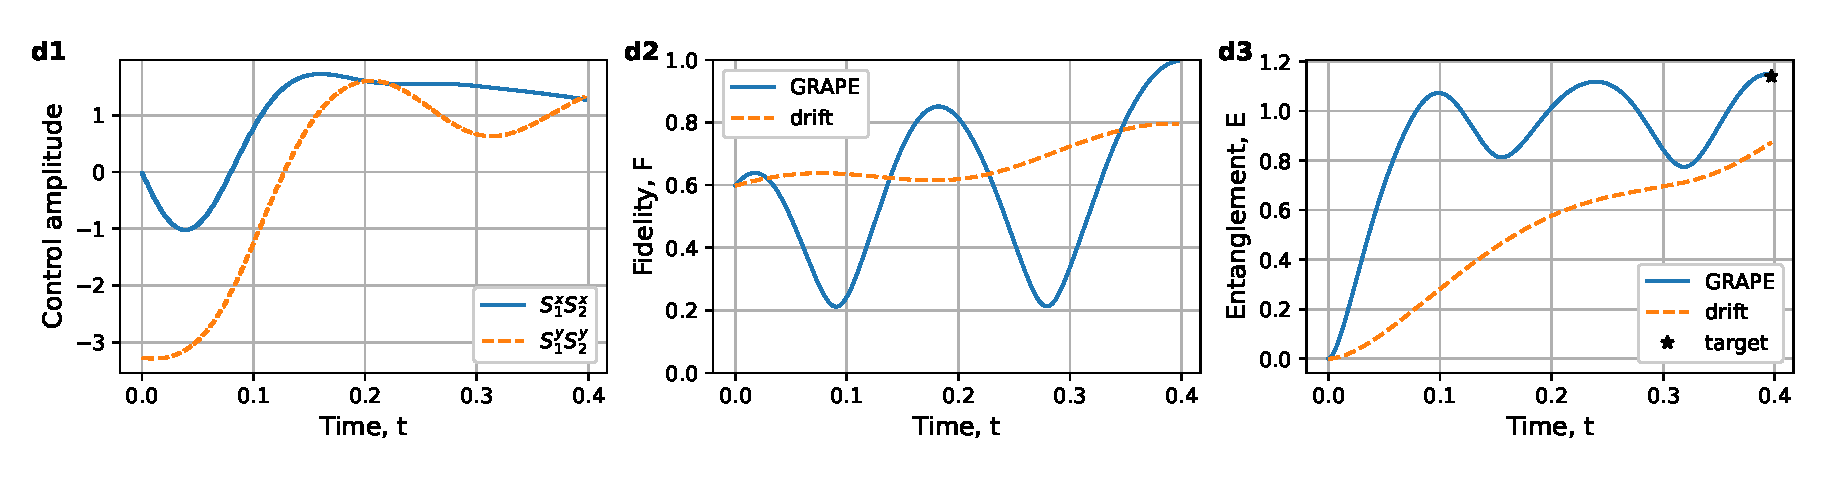
\includegraphics[width=0.92\textwidth]{fig3d.eps}
}
\captionstyle{normal}
\caption{
    Optimal control of {\bf a} $xx$ and $yy$ parts of $H_{2A2S}$ Hamiltonian separately and {\bf b}, {\bf c}, {\bf d} $H_{2A2S}$ Hamiltonian coupling constant during time {\bf a}, {\bf b} $\tau=\frac{2}{5\Omega}$, {\bf c} $\tau=\frac{1}{5\Omega}$ and {\bf d} $\tau=\frac{3}{10\Omega}$. In case {\bf c} and {\bf d} we also control rotation around $X$~-~axis. Amplitudes of the controls in controlled Hamiltonian are depicted in the left column {\bf a1}, {\bf b1}, {\bf c1} and {\bf d1}. Same qubit controls have similar amplitudes. A fidelity between the target state~(\ref{bosonqubitentanglement}) for $t=\frac{2}{5\Omega}$ and final state under the drift Hamiltonian itself and the full Hamiltonian obtained with GRAPE are depicted in the middle column {\bf a2}, {\bf b2}, {\bf c2} and {\bf d2}. Corresponded entanglement evolutions are depicted in the right column {\bf a3}, {\bf b3}, {\bf c3} and {\bf d3}.
}
\label{fig3:time-depended}
\end{figure*}

\newpage

\begin{figure*}[t!]
\setcaptionmargin{5mm}
\onelinecaptionsfalse
\subfigure{%
   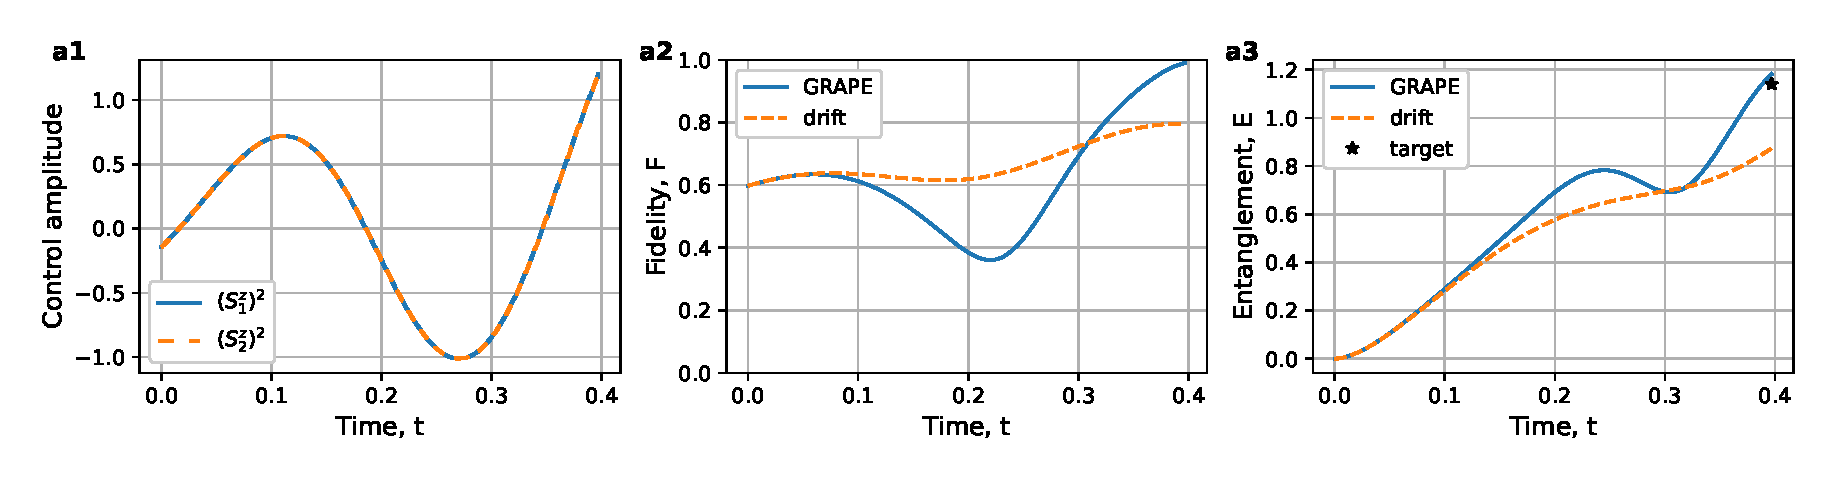
\includegraphics[width=0.92\textwidth]{fig4a.eps}
}
\subfigure{%
   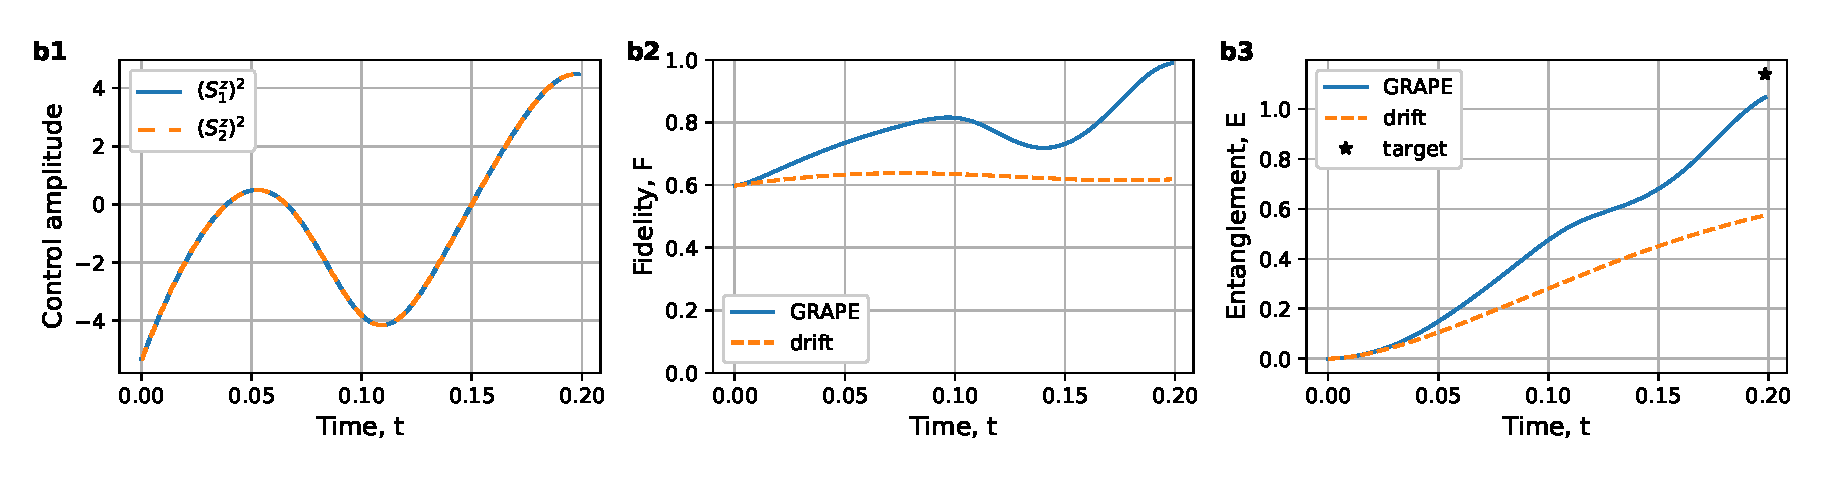
\includegraphics[width=0.92\textwidth]{fig4b.eps}
}
\subfigure{%
   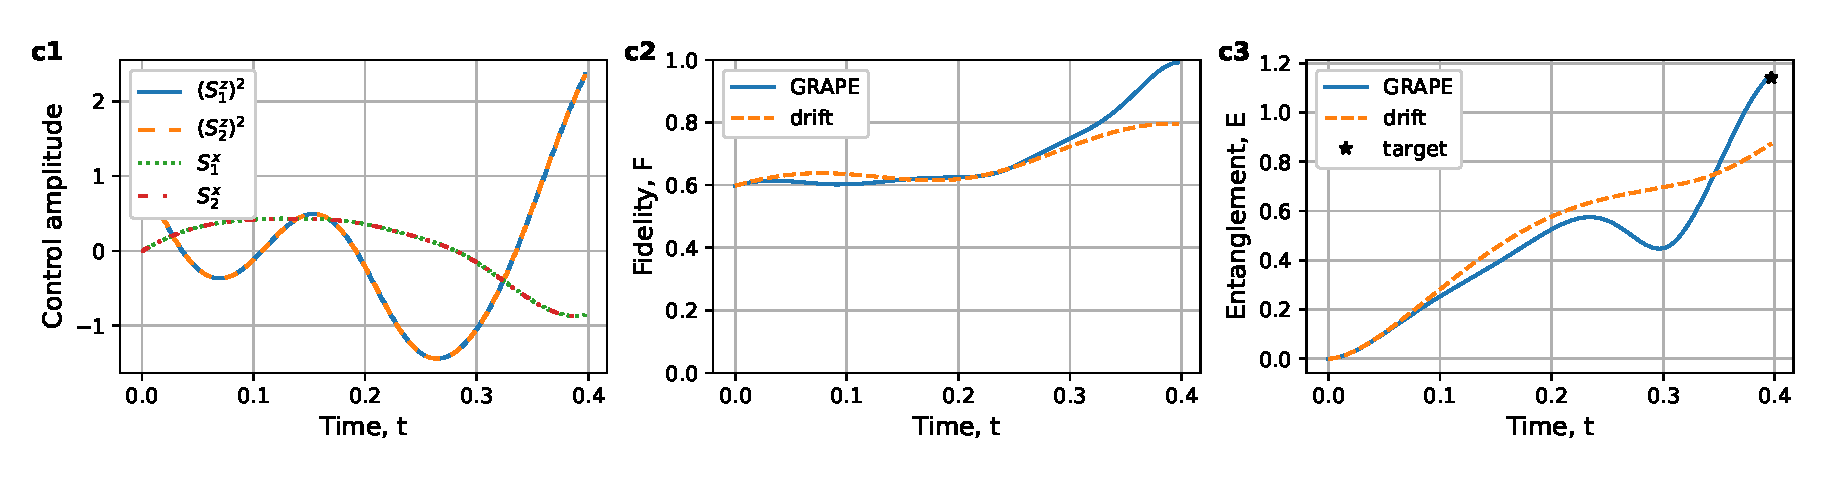
\includegraphics[width=0.92\textwidth]{fig4c.eps}
}
\captionstyle{normal}
\caption{
    Optimal control of squeezing $(S^z_i)^2$ ($i=1,2$) during time {\bf a}, {\bf b} $\tau=\frac{2}{5\Omega}$ and {\bf c} $\tau=\frac{1}{5\Omega}$. In case {\bf c} we also control rotation around $X$~-~axis. Amplitudes of the controls in controlled Hamiltonian are depicted in the left column {\bf a1}, {\bf b1} and {\bf c1}. Same qubit controls have similar amplitudes. A fidelity between the target state~(\ref{bosonqubitentanglement}) for $t=\frac{2}{5\Omega}$ and final state under the drift Hamiltonian itself and the full Hamiltonian obtained with GRAPE are depicted in the middle column {\bf a2}, {\bf b2} and {\bf c2}. Corresponded entanglement evolutions are depicted in the right column {\bf a3}, {\bf b3} and {\bf c3}.
}
\label{fig4:squeezing}
\end{figure*}

\newpage

\end{document}
